%!TEX TS-program = xelatex
%!TEX root = ../../maxwell2018thesis.tex

\chapter{Introduction}\label{chap:intro}
We live today in the so-called \emph{Information Age}, an era of human history characterised by the rapid development of technology allowing for the creation, transmission and retrieval of large volumes of information. Two key technological developments that have permitted such an increase in information generation are the computer and the associated technologies that allow for near-instantaneous communications with devices all around the planet, including the \emph{Internet} and~\gls{www}~\citep{berners1994www}. Indeed, with such technologies being  essentially ubiquitous in today's society, humankind today generates something in the range of \emph{2.5 quintillion bytes} of information \emph{per day}\footnote{$2.5$ quintillion bytes = $2,500,000,000,000,000,000$ bytes, or $2,500,000$ terabytes.}, according to a recent \emph{IBM} technical report\footnote{\url{https://www-01.ibm.com/common/ssi/cgi-bin/ssialias?htmlfid=WRL12345USEN} -- last accessed November 23\textsuperscript{rd}, 2017.}. To use a different unit of measurement, 250,000 times the amount of information held at the \emph{US Library of Congress}\footnote{This is calculated using the approximation on the US Library of Congress Blog, that says the Library holds the equivalent of 10 terabytes of information.}.

Sifting through such large volumes of information online to find the elusive and proverbial \emph{needle in the haystack} has been an area of active research and development over a number of decades. Since the early 1990's, the~\gls{www} has emerged as the dominant means of publishing information online over the Internet, replacing obsolete technologies such as the \emph{Gopher} protocol. As the amount of information available on the~\gls{www} grew\footnote{According to \url{http://www.internetlivestats.com/total-number-of-websites/}, there are over 800 million individual websites online today.}, so too did the paradigms employed by those wishing to seek information on it. Over the course of the first decade of the 21\textsuperscript{st} century, our approach to exploring the offerings on the~\gls{www} changed from the concept of \emph{surfing} a particular domain by following a series of hyperlinks, to the \emph{searching} of the ever-expanding universe of hyperlinked documents\footnote{Indeed,~\citep{mcbryan1994taming_tools} considered a search engine as a means of \emph{taming} the large number of online documents.}. Indeed, developing effective \emph{search engines} can be considered as the \emph{raison d'\^{e}tre} of the study of the study of~\gls{ir}.

\begin{quote}
    \emph{``...but perhaps the key technology that took the web from a useful supplement of current information practice to become the default communication medium is search.''}
    \attrib{\citealt*{wilson2010keyword_search}}
\end{quote}

Contemporary search engines such as \emph{Google} and \emph{Bing} are considered to offer an effective means of finding the proverbial needle in the haystack~\citep{wilson2010keyword_search}, where near perfect accuracy is regularly attained for popular \emph{queries}~\citep{vaughan2004new_measurements}. These search engines, along with the many others in existence today under a variety of different contexts, are the product of the collective work undertaken in the field of~\gls{ir} -- from early research in the 1970's~\citep{cleverdon1962cranfield_experiments,rijsbergen1979ir}; to the development of the various retrieval models that we use~\citep{robertson2009probabilistic_models}; to the setting up of evaluation forums~\citep{harman1993trec1}; to the development of the large-scale retrieval systems that we all use today~\citep{baezayates1999modern_ir, wang2010language_models}.

The work that the field of~\gls{ir} collectively undertakes is all done in the interests of making it easier for potential users of search engines to satisfy their underlying \emph{information need}. Arriving with an \emph{anomalous state of knowledge}~\citep{belkin1980ask}, a searcher then formulates a \emph{query} -- an expression of what they are looking for~\citep{borlund2003iir_model} -- before being presented with a potentially relevant set of documents. However, the interactions that take place between a searcher and a search engine are complex~\citep{ingwersen2005theturn}. This process, where the searcher engages in \emph{dialogue} with the search system, is considered the study of~\gls{iir}~\citep{borlund2003iir_model}.

\section{Motivation and Context}
Central to much of the work undertaken in the field of~\gls{ir} over the past 50 years is the so-called \emph{Cranfield Paradigm}, which denotes a standardised approach for the evaluation of~\gls{ir} systems. The Cranfield paradigm descends directly from \emph{Cranfield II}~\citep{aslib1966factors}, a set of experiments designed to evaluate the efficiency of indexing systems. At the time, searching for information on computer systems was achieved through the issuance of queries to a \emph{boolean retrieval system}, with terms matched against a small set of manually indexed documents~\citep{harman2010cranfield}. Included is a set of \emph{relevance judgements} for each of the documents, as judged by humans, allowing one to then ascertain the performance of a given search system.

While the basic principles of the Cranfield Paradigm have remained in place since it was established in the 1960's, components of the approach have evolved over the years to cater for the ever increasing complexity of the tasks at hand~\citep{harman2010cranfield}. Indeed, the approach is still widely used in evaluation forums, such as the \emph{NIST}-sponsored \emph{Text REtrieval Conference (TREC)} -- the first of which was held in 1993~\citep{harman1993trec1}. Indeed, many of the \emph{relevance assessments} and \emph{topics} provided as part of \emph{TREC Tracks} over the years are used as ground truths throughout the work discussed in this thesis.

The approach however can be argued to remain simplistic in terms of when considering the complex user interactions that take place during the search process~\citep{borlund2000evaluation_iir,ingwersen2005theturn}. In other words, the Cranfield Paradigm broadly fails to consider the complexities of the~\gls{iir} process, where, for example, searchers can issue multiple queries during the course of a search session, and adapt their interactions baed upon the perceived quality of the presented rank list of results for each associated query~\citep{moffat2013users_versus_models}. Selecting good terms to use within a query is difficult yet important~\citep{efthimiadis2000query_expansion}; as such, the initial query posed in a search session often acts as an entry to the search system, followed by phases of browsing and query reformulations~\citep{marchionini1993information_seeking}. Therefore, the first query formulation of the user often acts as an entry to the search system followed by subsequent phases of browsing and query reformulations (Marchionini et al. 1993). Searchers also will typically abide by the principle of least effort -- striving to minimise the probable average rate of work expenditure over time~\citep{zipf1949behaviour}. Cranfield considers that a user will \emph{(i)} issue a single query; \emph{(ii)} examine documents to a large depth (typically $1,000$ documents); and \emph{(iii)} consider all documents to be relevant. This is largely unrealistic, and numerous researchers have proposed alternatives to the Cranfield Paradigm, such as~\citealp{borlund2003iir_model}.

\citealp{keskustalo2008user_simulation} categorised~\gls{iir} research into four different approaches that allow for the consideration of the complex interactions that take place between a human and the search engine being used. These are:

\begin{itemize}
    \item[\blueboxbold{1}]{the observation of real-world searchers, in real world scenarios (e.g. general web search), through the use of interaction logs;}
    \item[\blueboxbold{2}]{the observation of real-world searchers undertaking simulated work tasks in a lab-based environment;}
    \item[\blueboxbold{3}]{performing \emph{simulations} of interaction in a lab-based environment, sans real-world searchers; and}
    \item[\blueboxbold{4}]{the undertaking of \emph{traditional} lab-based experimentation.}    
\end{itemize}

Obtaining interaction data from studies utilising real-world users undertaking search tasks (categories \blueboxbold{1} and \blueboxbold{2}) will of course always be the preferred option. However, there are pitfalls with both approaches that must be considered, primarily in terms of \emph{availability} and \emph{cost}. Obtaining data for studies conducted in category \blueboxbold{1} is difficult if the researchers do not work for an organisation offering a large-scale, search engine. Working within an academic setting for example may greatly restrict what data can be obtained. Indeed, working with real-world interaction data also leads to major ethical and privacy concerns~\citep{korolova2009aol_query_log_privacy}. The release of the \emph{AOL Query Log} (and subsequent fallout) in August 2006 is testament to that, although this has not stopped researchers from utilising the data in their work (e.g.~\citealp{brenes2009aol_query_log}).

This will leave many researchers with category \blueboxbold{2}. While this approach also leads to the capturing of real-world interaction data, pitfalls of this approach primarily are the significant costs involved in such an approach -- both financially and in terms of time. Considerations must also be placed into study design to mitigate potential biases as much as possible. In recent years however, the concept of \emph{crowdsourcing} may alleviate some of these concerns, and open up a potential study to a larger potential audience. A recent study has shown that using crowdsourcing to capture interaction data is no worse than a carefully controlled lab-based user study~\citep{zuccon2013crowdsourcing_comparisons}, although quality control measures must be taken.

While categories \blueboxbold{1} and \blueboxbold{2} provide real-world interaction data, options \blueboxbold{3} and \blueboxbold{4} do not. Such approaches however, if executed correctly, can potentially lead to insights that would not otherwise be possible when involving real-world users. As an example, covering an extensive set of test cases may simply not be possible~\citep{keskustalo2008user_simulation} -- perhaps due to financial constraints, or a lack of suitable subjects. Category \blueboxbold{4} can be considered as a means of conducting \emph{traditional, TREC-style}~\gls{ir} lab experimentation that is, as previously mentioned, largely na\"{i}ve of the user's complex interactions. This leaves category \blueboxbold{3} as a means of conducting and evaluating user-sided experimentation without the explicit need for real-world users to be present. This approach uses \emph{simulation} as a means to conducting such experiments.

\subsection{Why Simulation?}
Simulation is defined as the \emph{imitation of the operation of a real-world process or system over time}~\citep{banks1996discrete}. Such an approach allows one to gain insight into the functioning of some real-world phenomenon. Simulation has been used in a wide range of areas, including, for example, examining physical processes~\citep{haessig1991physics_modelling}, psychology~\citep{hastie1988human_memory_simulation}, road traffic~\citep{mahmud2016traffic_modelling_electric} and training for various activities, such as piloting an aeroplane~\citep{sparko2010flight_simulators}. Central to contemporary uses of simulation if the idea \emph{computerised simulation}~\citep{heermann1990computer_simulation}, thanks to ever increasing computational power available for such tasks -- such as the simulation of racing cars for the purposes of driver development, as shown in Figure~\ref{fig:ch1-mclaren}. In summary, employing simulation provides a rapid means of exploring the components, all at a low cost -- all while permitting repeatable, and therefore reproducible, results~\citep{maxwell2016agents}.

One of the key components of any simulation -- regardless of whether it is executed on a computer or not -- is that of an underlying \emph{model} of the real-world phenomenon being simulated~\citep{tocher1963art_of_simulation}. This model defines the various stages, rules and other descriptive components of the phenomenon that simulations must consider. These rules are often high level, and as such, a number of \emph{assumptions} are made~\citep{tocher1963art_of_simulation}. For example, the TREC Paradigm assumes that a single query is issued by a searcher within a search session, and searchers examine to great depths per query. These assumptions should be made in the face of supporting evidence; evidence in IIR studies strongly suggests that searchers do not follow this rigid approach, but rather adapt their behaviour based upon the proximal cues presented to them.

Why though, use simulation when other alternatives to modelling the search process are available? Alternatives include some form of closed-form system, such as a series of linear equations to describe the complex interactions that take place. However, according to~\citealp{fishwick1995simulation}, this approach is not flexible enough, and lists a number of reasons as to why simulation is essential in complex, dynamic systems:

\begin{itemize}
    \item{the model is very complex, with many variables and interacting components;}
    \item{the underlying variables and relationships are non-linear;}
    \item{the underlying models contains random variates; and}
    \item{the model output is to be visual, as in a three-dimensional computer animation.}
\end{itemize}

In the context of~\gls{iir}, the first three reasons can be considered as acceptable reasons for why simulation is an advantageous methodology to pursue. For example, many state-of-the-art~\gls{iir} models consider a stochastic component when determining the relevancy of a document to a particular topic.

Simulation provides a means of using a uniform model execution technique that can be used to solve a large variety of systems, without resorting to a ``bag of tricks'', where one must choose special-purpose and sometimes arcane solutions to avoid simulation~\citep{fishwick1995simulation}. Simulation provides the freedom and flexibility to permit the implementation of a model that better represents the real-world phenomenon that is being considered. In contrast, with a more closed-form approach, the underlying model that is created is often twisted and altered to suite the closed-form approach, rather than to actually represent the real-world system. This leads to a larger gap between the model and reality, and as such leads to a greater number of assumptions within the model than what would otherwise be required. In other words, the technique used to develop the model constrains just how realistic is can be.

\begin{figure}[t!]
    \centering
    \resizebox{1\hsize}{!}{
    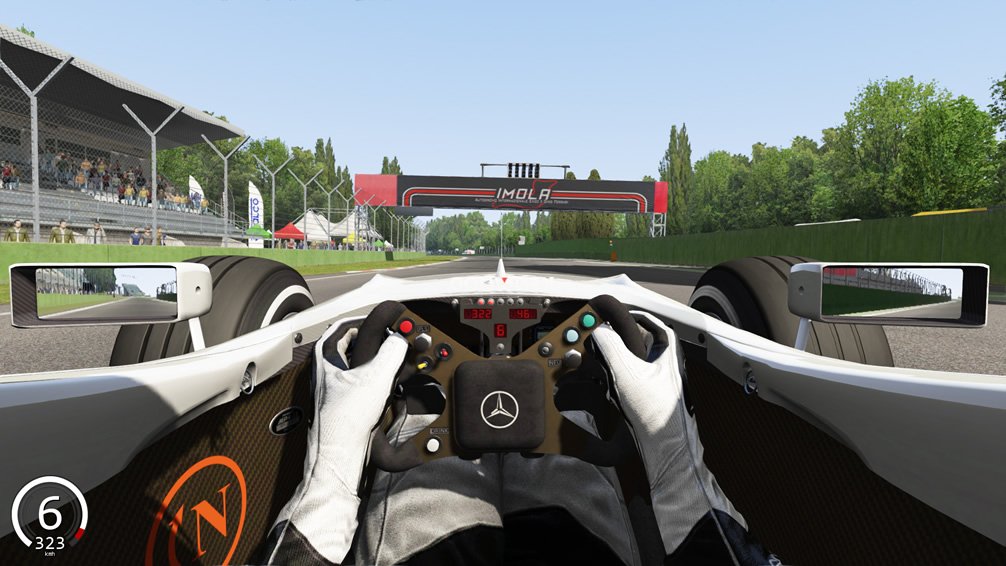
\includegraphics{figures/ch1-mclaren.jpg}}
    \caption[Racing Simulator Example]{An example of a \emph{video game simulation}, \emph{Assetto Corsa}. In this figure is a model of the \emph{McLaren-Mercedes MP4/13} race car, driving around the \emph{Autodromo Enzo e Dino Ferrari} race track in the \emph{Emilia-Romagna} region of Italy. In the past ten years, the increase in computing power in CPUs and GPUs has enabled the development of increasingly complex (and \emph{more realistic}) video game simulations, which, for example, are now used in the training of racing drivers.}
    \label{fig:ch1-mclaren}
\end{figure}

As a means to providing better and more flexible models, simulation has been used extensively within~\gls{ir}, such as the simulation of work tasks and tracks, simulated and synthetic data collections, and of course \emph{simulated interaction}, which is what this thesis considers. While this encapsulated category \blueboxbold{3} of the four categories as outlined by~\citealp{keskustalo2008user_simulation}, we also argue that in order to run simulations of interaction, they must be \emph{grounded} using real-world observations, which in turn means the assumptions that are made in the simulated model can be considered to be a credible abstraction of the real-world phenomenon. As such, this necessitates access to data obtained through either categories \blueboxbold{1} or \blueboxbold{2} -- and without access to a large-scale search engine, this leaves category \blueboxbold{2} as means for acquiring such data. As such, this thesis presents the \emph{Complex Searcher Model (CSM)} as a means of modelling the IIR process, with each component grounded using interaction data from a number of user studies, also conducted as part of this thesis. Of particular interest within this model is the concept of \emph{stopping behaviour} (e.g. \emph{how far down this ranked list of results should I go?}).

\subsection{Why Stopping?}
Knowing when to stop is a fundamental aspect of human thinking, with individuals commonly employing some form of \emph{stopping criterion} to decide when they should stop with their interactions in the world around them~\citep{nickles1995judgment}. As an example, a shopper looking to buy a new smartphone will stop shopping around once he or she has obtained sufficient information on what new device to purchase. A doctor, once their case notes about a patient's condition have been finished, will then diagnose their ailment. In the context of search, stopping may be considered at a variety of different points during the search process. The commonly used example of \emph{search stopping behaviour} is the point at which a searcher should stop examining a list of ranked results, or, in other words, \emph{how far down the ranked list the searcher should go}, for example.

The decision of when to stop is not necessarily due to external factors, but from a series of \emph{internal factors} of the decision maker's thinking process. In the context of informational search, knowing when to stop requires that the individual makes a judgement regarding the sufficiency of the information obtained, and whether or not additional information is required to be obtained~\citep{browne2004stopping_rules}. This is normally characterised by both the completeness and correctness of the information obtained thus far~\citep{smith1991belief}. These claims can be mirrored by qualitative studies on examining stopping behaviour, where researchers have found that searchers stop examining a ranked list of results simply because what they have found previously is \emph{``good enough''}~\citep{wu2014information_scent}.

Considering the above, is there any means by which we can quantify what this feeling of \emph{``good enough''} actually is? Researchers have devised a series of different \emph{stopping heuristics} as a means to try and encapsulate the differing stopping behaviours exhibited by searchers. However, the literature in examining which of these heuristics offers the best approximations to what searchers actually do is somewhat limited. By focusing on stopping behaviour within this thesis, our model provides additional points at which a simulated user can stop interactions with a search engine, and thus save time and effort that might otherwise have been wasted if they continued to examine content.

\vspace{-5mm}
\section{Thesis Statement}
The statement of this thesis is that by considering various \emph{stopping decision points} within model representing a user's interactions during the search process, one can run simulations of interaction that offer a greater degree of realism -- and thus a better approximation of the actual behaviours exhibited by real-world searchers -- than currently employed models.

In particular, incorporating such stopping decision points within a representation of the search process will allow the simulated user following such a model a greater degree of flexibility -- allowing them, for example, to abandon a set of results that is judged to be of low relevancy to the given query. In addition, these decision points can be instantiated by operationalising a series of different \emph{stopping heuristics} that attempt to encapsulate the stopping behaviours exhibited by real-world searchers. Furthermore, by taking this knowledge forward, we can then apply grounded simulations over a variety of different search contexts, examining how stopping behaviour of real-world searchers varies under each context -- and through simulation, we can then deduce what particular heuristic(s) offer the best approximation to searcher behaviours.

\section{Overarching Research Questions}
From the introductory remarks, motivation and thesis statement provided previously in this chapter, we can now formulate the three main research questions that this thesis addresses. 

\begin{itemize}

    \item[]{\blueboxbold{HL-RQ1} Considering stopping behaviours, can we improve upon and make \emph{more realistic models} of the~\gls{iir} search process -- as a whole?}

    \item[]{\blueboxbold{HL-RQ2} How can we operationalise and subsequently implement more realistic stopping strategies for use within many of the commonly used~\gls{ir} and~\gls{iir} models and measures that are in use today?}

    \item[]{\blueboxbold{HL-RQ3} How do the real-world stopping behaviours of searchers vary under different contexts?}

\end{itemize}

\section{Origins of the Material}
Material presented in this thesis has appeared previously in several conference papers. All of these papers were published throughout the duration of this PhD programme (2013-2018). The list below details each of the publications in chronological order.

\begin{itemize}
    \item{\bibentry{maxwell2014temporal_delays}}
    \item{\bibentry{maxwell2015initial_stopping}}
    \item{\bibentry{maxwell2015stopping_strategies}}
    \item{\bibentry{maxwell2016dc}}
    \item{\bibentry{maxwell2016simiir}}
    \item{\bibentry{maxwell2016agents}}
    \item{\bibentry{maxwell2017snippets}}
\end{itemize}

\section{Thesis Contributions}
This thesis offers four main contributions to the research community, revolving around the concepts of user modelling and stopping behaviours during search.

\begin{itemize}
    \item[\blueboxbold{C1}]{We provide a series of contributions on user modelling within the IIR process. Specifically, we focus on the development of accepted user models by incorporating additional \textbf{stopping decision points}, and incorporating the ability for a simulated user to remember what has been examined through the inclusion of some basic \textbf{form of state}.}
    
    \item[\blueboxbold{C2}]{The second main contribution is the \textbf{SimIIR framework}, developed to allow for the running of \textbf{simulations of interaction}. Within the framework, our proposed user model is encoded, along with the ability to specify and configure various components of the search process. An explanation of the framework is provided in Appendix~\ref{appx:simiir}.}
    
    \item[\blueboxbold{C3}]{We provide a comprehensive survey on various s\textbf{topping heuristics} that have been proposed over the years in the literature, before providing analysis on how performance and behavioural characteristics vary when considering:}
    
    \begin{itemize}
        \item{Snippet-Level stopping and associated strategies;}
        \item{SERP-Level stopping; and}
        \item{Session-Level stopping.}
    \end{itemize}
    
    \item[\blueboxbold{C4}]{Finally, we provide analysis examining how the \textbf{stopping behaviour of searchers varies under different search contexts}, such as when we vary the overall search goal, or vary presentational aspects of the presented results.}
    
\end{itemize}

\section{Remaining Thesis Outline}

% \todo{======}
%
%
%
%
% \section{Motivation and Context}
% Central to the~\gls{ir} community is the so-called \emph{Cranfield Paradigm}, which represents a standardised approach for the evaluation of~\gls{ir} systems. The paradigm was designed in the early 1960's, when information access was largely achieved through the issuance of boolean queries against manually indexed documents~\citep{harman2010cranfield}. Initial experiments, known as the \emph{Cranfield Experiments}~\citep{cleverdon1962cranfield_experiments}, focused on a single query and associated relevance judgements.
%
% While explained in more detail in Chapter~\ref{chap:background}, the Cranfield paradigm has remained in use to this day, being the \emph{de facto} approach employed by various~\gls{ir} evaluation forums, such as the \emph{NIST}-sponsored \emph{Text REtrieval Conference (TREC)}. Indeed, many of the \emph{relevance assessments} and \emph{topics} provided as part of \emph{TREC Tracks} over the years are used as ground truths throughout the work discussed in this thesis. While components of the paradigm have evolved over the decades as underlying tasks have become more complex~\citep{harman2010cranfield}, the approach however can be argued to remain simplistic in terms of when considering the complex user interactions that take place during the search process~\citep{ingwersen2005theturn, borlund2000evaluation_iir}. In other words, the Cranfield Paradigm broadly fails to consider the complexities of the~\gls{iir} process, where, for example, searchers adapt their interactions baed upon the perceived quality of the presented rank list of results~\citep{moffat2013users_versus_models}.
%
%
% A searcher approaches an Information Retrieval (IR) system with a need for information derived from an ‘anomalous state of knowledge’ (Belkin et al., 1982). This need is typically transformed into a query statement, submitted to the system and a set of potentially relevant documents is retrieved and presented. The transformation of this need into a search expression, or query, is known as query formulation. Through such transformations and further interaction searchers can conduct Interactive IR (IIR), where they engage in dialogue with the IR system and it dynamically responds to their feedback (Borlund, 2003).
%
%
% ~\citep{borlund2003iir_model}
%
%
%
%
% Central to the Information Retrieval community is the so-called Cranfield Paradigm, having been established since the 1960's. This approach leads to reproducibility of experiments, and sensible approach to providing a means of evaluation for improvements of ranking algorithms, for example. Indeed, this approach is still widely used in IR today. Every year, TREC uses this approach. NTCIR and other TREC-inspired conferences use this approach. The approach provides the community with document assessments, which are difficult to procure, and promotes that reproducibility.
%
% What about the user? In an age where information is expected to be found almost instantaneously, people demand a search engine that works. And indeed, we broadly do have that in \emph{Google} -- as per Max Wilson. But do we really have a solid understanding of the complex interactions that take place between a searcher and a human? The field of IIR tries to address this gap in our knowledge.
%
% a user will typically abide by the principle of least effort -- striving to minimise the probable average rate of work expenditure over time (zipf, 1949)
%
% This need is typically transformed into a query statement, submitted to the system and a set of potentially relevant documents is retrieved and presented. The transformation of this need into a search expression, or query, is known as query formulation. Through such transformations and further interaction searchers can conduct Interactive IR (IIR), where they engage in dialogue with the IR system and it dynamically responds to their feedback (Borlund, 2003).
%
% IIR is a complex process in which people issue a multiple queries in a session (The Turn). One central argument is that the Cranfield Paradigm is essentially na\"{i}ve of the complex interactions that take place. Cranfield can be considered to issue a single query, typically the title of a topic, and examine to a large depth (typically 1000), while assuming that all documents are relevant. We know, as humans, that this is not representative of real-world searchers. We know that searchers adapt their behaviour due to a variety of factors, perhaps most notably due to the perceived quality of the returned list of ranked results. They \emph{adapt}. TREC users do not.
%
% When considering users, a number of different approaches have been considered. Keskustalo
%
% \begin{itemize}
%
%     \item[\blueboxbold{1}]{the analysis of log data collected from real-world scenarios (e.g. from commercial web search engines);}
%     \item[\blueboxbold{2}]{the collection of interaction data from simulated search tasks (e.g. a lab-based user study);}
%     \item[\blueboxbold{3}]{the simulation of interaction, considering the user and the various processes that are undertaken -- sans users -- and}
%     \item[\blueboxbold{4}]{`traditional' lab-based studies, sans users, aka TREC-style experimentation.}
%
% \end{itemize}
%
% IR experiments regarding user simulations may be classified into four classes: (i)
% observing users in real situations (i.e., real users; no simulation), see, e.g., Spink and
% Saracevic (1998); (ii) observing users performing simulated tasks (e.g., Belkin et al. 1995);
% (iii) performing simulations in the lab without users (simulation; no users) (e.g., Keskustalo
% et al. 2006; White et al. 2004); and (iv) traditional lab research (no users and no simulation
% point of view regarding user attributes or user action). Studies on real users performing real
% or simulated RF tasks provide realistic and rich data but it is difficult to cover extensively
% numerous test cases. On the other hand, laboratory studies typically do not model users
% explicitly, though they can be seen as abstractions of user searching (e.g., Rocchio 1971).
% Our goal in this paper is to extend the lab model towards the user point of view and
% perform user simulations in the lab (without users) to explore explicitly the consequences
% of variation in user’s feedback behavior (class (iii) above).
%
% Now we need a thorough explanation of each point.
% Which leaves option (3) as the remaining approach. This thesis considers simulation and user modelling. argue that in order to undertake number (3), you also need to acquire some real-world data, through means described as options (1) or (2). this is exactly what this thesis attempts to address.
%
%
% \subsection{Why Simulation?}
% - from that online thing, why do simulation? why not just make a mathematical model instead?
% - low cost, etc. easy to experiment with.
% - overheads are power consumption, etc.
% - little bit of explanation of simulation, what it can be used for. not just on a computer!
%
% - in the domain of IIR, simulation has been used for a variety of different contexts, such as simulating
%
% - components have been considered in isolation. like query generation. other approaches consider the search session as a whole -- a very complex approach indeed.
%
% - in order to simulate, you need a model of the phenomenon that you are examining.
%
% \subsection{User Modelling}
% - cognitive models etc
%
% - different components in a model.
% - but what about stopping?
%
% \subsection{Why Stopping Behaviour?}
% - fundamental aspect of human thinking.
% - we do it in everything we do -- otherwise we wouldn't stop!
% - search is no exception. how many results should I examine? how many queries should I issue?
%
% - this is hugely dependent upon a variety of factors, such as task type, environmental factors...etc...
% - but the fundamental point is that stopping is a crucial behaviour to help in developing our understanding of \emph{how people search.}
%
% - work in this area has been until recently relatively sparse.
% - user sided and system sided
% - user sided dealing with simply what is ``good enough''. But what is this feeling of good enough?
% - rules since the 1970's in IR journals, ecology journals...
% - can we take these rules and implement them in some way to examine stopping behaviour?
%
% \section{Thesis Statement}
% The statement of this thesis is that by considering the stopping behaviour of searchers, we are able to obtain a better understanding of how people search, through the use of user modelling. Specifically, we can use simulation to enhance our understanding of the behaviours people exhibit under certain conditions. Work in this area leads to the notion of \emph{agency}.
%
%
% \section{Overarching Research Questions}
%
% \section{Origins of the Material}
% Material presented in this thesis has appeared previously in several conference papers. All of these papers were published throughout the duration of this PhD programme (2013-2018). The list below details each of the publications in chronological order.
%
% \begin{itemize}
%     \item{\bibentry{maxwell2014temporal_delays}}
%     \item{\bibentry{maxwell2015initial_stopping}}
%     \item{\bibentry{maxwell2015stopping_strategies}}
%     \item{\bibentry{maxwell2016dc}}
%     \item{\bibentry{maxwell2016simiir}}
%     \item{\bibentry{maxwell2016agents}}
%     \item{\bibentry{maxwell2017snippets}}
% \end{itemize}
%
% \section{Thesis Contributions}
%
% \section{Thesis Outline}
%
% %%%%%%%%%%%%%%%%%%%%%%%%%%%%%%%%%%%%
% %
% % People are often exposed to more information than they can remember~\cite{murayama2016enough_is_enough}. But when do they stop?
% %
% % The volume of information available at our fingertips is ever increasing. Despite the huge advances in the underlying systems that we now rely upon on a daily basis, we still lack a thorough understanding of the \emph{Human-Computer} link. What does it mean when a searcher abandons their query? Does it mean they are satisfied? Maybe it does, maybe it doesn't. Regardless of this, we still have a lot of work to understand the behaviours exhibited by searchers when examining information. This thesis attempts to plug the gap, even just a little bit.
% %
% % \section{Motivation}
% % The \emph{Information Retrieval (IR)} community has centred much of its recent research upon the so-called \emph{Cranfield Paradigm}. The paradigm revolves around the idea of a test collection and associated relevance judgements for documents within said collection. This approach provides a standardised way in which one can evaluate their retrieval system against a given baseline. While the general concepts of the paradigm have remained in place since the 1960s, components have over the years evolved as the associated data and tasks have become ever more complex in nature~\cite{harman2010cranfield}. Examples of use today include the \emph{NIST}-sponsored \emph{Text REtrieval Conference (TREC)} and other evaluation forums.
% %
% % The Cranfield Paradigm today still largely remains the \emph{de facto} means of IR evaluation. Despite this however, the approach possesses a simplistic means of examining the actions with which a real-world searcher undertakes. As such, several different scientific approaches have been developed to better understand the complex sequence of interactions taking place, and are readily used in the study of \emph{Interactive Information Retrieval (IIR)} which deals specifically with the interactions between humans and search engines. As outlined by~\citeauthor{keskustalo2008user_simulation}~\cite{keskustalo2008user_simulation}, the approaches can be split into four distinct categories:
% %
% % \begin{itemize}
% %     \item{obtaining data from searchers in real-world situations (e.g. log data from a commercial search engine);}
% %     \item{observing searchers perform simulated search tasks (e.g. a user study involving a search engine);}
% %     \item{performing simulations in a lab environment (e.g. simulations of interaction, without real-world searchers); and}
% %     \item{traditional lab-based research, sans real-world searchers.}
% % \end{itemize}
% %
% % Experimentation with real-world searchers undertaking either real or simulated search tasks is the preferred way to study IIR (approaches \emph{\textbf{1}} and \emph{\textbf{2}}). However, such experiments require a significant level of effort to organise and setup. They are also laborious to run, and are usually very costly - both for the researcher and subject involved~\cite{azzopardi2010workshop}. Approach \emph{\textbf{4}} can be argued as a simplistic form of \emph{`TREC-style'} simulation, assuming a single query with a fixed number of documents examined in a linear fashion. This approach however is not interactive, and can be considered na\"{i}ve.
% %
% % %Lab-based studies (approach \emph{\textbf{4}}) may be seen as limited-perspective abstractions of user search. However, contrary to the argument by~\citeauthor{keskustalo2008user_simulation}~\cite{keskustalo2008user_simulation}, this particular form of research can be considered a very simplified form of \emph{`TREC-style'} simulation. Here, assumptions include a single query, with up to 100 documents examined in a linear fashion. This approach is not interactive and na\"{i}ve.
% %
% % %Furthermore, if several rounds of experimentation are required, a larger pool of subjects are required due to the effects of fatigue and learning bias
% %
% % This therefore leaves the simulation of real-world searchers, incorporating \emph{interactive} components such as relevance feedback and other interaction components (approach \emph{\textbf{3}}) as a means of exploring IIR. As the main focus of this project, simulation provides a rapid means of exploring the potential limits of real-world searcher interactions at a low cost. Current means of simulation are limited because they assume searchers act in a fixed way, or act stochastically by examining content with fixed probabilities. Research has shown that in reality, searchers tend to adapt their interactions based upon the quality of the presented ranked list~\cite{moffat2013users_versus_models}. Simulations of course would not be effective if the underlying models and assumptions do not adequately represent the actions that real-world searchers would be inclined to undertake~\cite{azzopardi2010workshop}. While the IIR community has recently made advances in user modelling (e.g.~\cite{azzopardi2011economics, azzopardi2014economics, baskaya2013behavioural_factors, thomas2014modelling_behaviour}), a significant amount of work is still required to make simulations of searchers more credible. To this end, this project aims to build more realistic simulations, starting with a \emph{Complex Searcher Model (CSM)}, illustrated as a flowchart in Figure~\ref{fig:csm}. Within the CSM, a complex search process is modelled, where each component (e.g. query generation) and decision point (e.g. deciding when to stop) can be varied and customised. We also instantiate the CSM with components grounded from empirical evidence based upon actual real-world searcher behaviour and interaction data, providing realism to the simulations.
% %
% % This therefore leaves the simulation of real-world searchers, incorporating \emph{interactive} components such as relevance feedback and other interaction components (approach \emph{\textbf{3}}) as a means of exploring IIR. As the main focus of this project, simulation provides a rapid means of exploring the potential limits of real-world searcher interactions at a low cost (i.e. a real-world searcher would be unlikely to examine 100 documents - but this would not be an issue with simulation). Simulations of course would not be effective if the underlying models and assumptions do not adequately represent the actions that real-world searchers would be inclined to undertake~\cite{azzopardi2010workshop}. While the IIR community have recently made advanced in user modelling (e.g.~\cite{azzopardi2011economics, azzopardi2014economics, baskaya2013behavioural_factors, thomas2014modelling_behaviour}), a significant amount of work is still required to make simulations of searchers more credible. To this end, this project aims to build more realistic simulations, using a \emph{Complex Searcher Model (CSM)}, as illustrated in Figure~\ref{fig:csm}. Within the CSM, each component (e.g. query generation) and decision point (e.g. deciding when to stop) can be varied and customised. We also instantiate the CSM with components grounded from empirical evidence based upon actual real-world searcher behaviour and interaction data. This therefore provides the simulations with realism and credibility.
% %
% % \begin{figure}[t!]
% %     \begin{center}
% %     %\vspace{-2mm}
% %     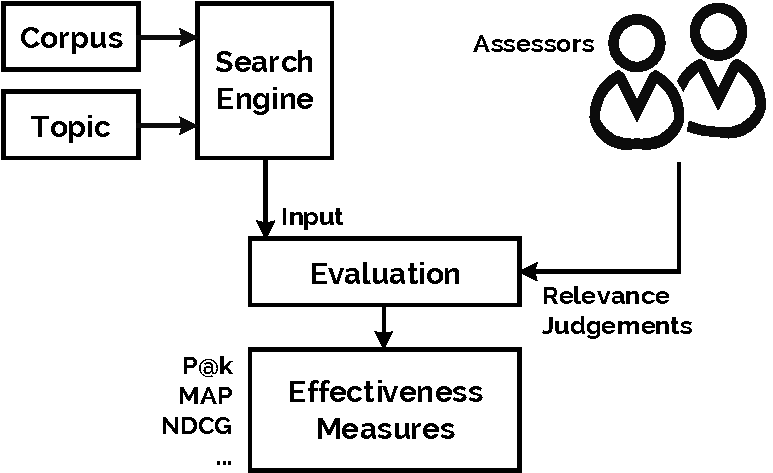
\includegraphics[width=\linewidth]{figures/cranfield.pdf}
% %     \caption{The Cranfield Paradigm. Document collections (corpora) and associated topics are created, and are then passed to assessors to judge the relevancy of documents against the provided topics. These judgements are then provided to researchers as \emph{relevance judgements}, which are then used to evaluate the performance of retrieval components with different \emph{effectiveness measures}, such as \boldmath{$P@k$}.}
% %     \label{fig:cranfield}
% %     \end{center}
% % \end{figure}
% %
% % \subsection{Why Simulation?}
% % A question that readers of this thesis may ask early on is: \emph{why use simulation?} Could the behaviours exhibited by human searchers instead be perhaps modelled through less computationally intensive means? This is a perfectly valid question to ask; indeed, the author tripped up when asked this question at the 1\textsuperscript{st} ACM CHIIR Doctoral Consortium.
% %
% % One of the potential criticisms of this work is: why simulate at all? Why not just plug everything into an equation, and solve it? \url{https://www.cise.ufl.edu/~fishwick/introsim/node2.html}
% %
% %
% % \section{Thesis Statement}
% %
% % - statement of fact: users are complex, and adapt their behaviour due to a variety of different factors, not limited to the ranked list of results presented to them.
% % - statement of fact: many of the models and measures that we use in IR do not assume this.
% % - one thing we do not consider much is stopping behaviour. by incorporating stopping behaviour into our models, we can provide better approximations of searcher behaviour
% %
% % - The statement of this thesis is that incorporating stopping level decision points into a user model will lead to more efficient searching, and better approximations of actual searcher behaviour
% %
% %
% % The statement of this thesis is that we can improve our understanding of the stopping behaviour of searchers through experimentation. This understanding can be further improved through the use of simulation.
% %
% %
% % \section{Overarching Research Questions}
% % From the introductory remarks, thesis statement and motivation as described above, we can now formulate the three main research questions that will be addressed in this thesis.
% %
% % \begin{itemize}
% %
% %     \item[]{\blueboxbold{RQ1} How can we improve upon and make \emph{more realistic models} of the~\gls{iir} search process -- as a whole?}
% %
% %     \item[]{\blueboxbold{RQ2} How can we operationalise and subsequently implement more realistic stopping strategies for use within many of the commonly used~\gls{ir} and~\gls{iir} models and measures that are in use today?}
% %
% %     \item[]{\blueboxbold{RQ3} How do the real-world stopping behaviours of searchers vary under different contexts?}
% %
% % \end{itemize}
% %
% % Each of these research questions will be addressed in parts \blueboxbold{I} and \blueboxbold{II}.
% %
% % \section{Contributions}
% % The work undertaken towards completion of this thesis has led to a number of contributions to the field, many of which have been published in international conference proceedings. The following contributions have been made.
% %
% % \begin{itemize}
% %
% %     \item{An extensible simulator framework, called \emph{SimIIR}, that allows for full-session~\gls{iir} simulation.}
% %
% %     \item{The introduction and evolution of the Complex Searcher Model, a full-session model of the~\gls{iir} process. Note that this model does not attempt to model the brain; rather, it is a model of the overarching steps and decisions that a searcher makes during the search process. We do model state; this does not consider the brain, nor does the model consider other issues such as environmental factors.}
% %
% %     \item{A series of user studies that examine the effects of stopping behaviour on:}
% %
% %     \begin{itemize}
% %         \item{temporal delays;}
% %         \item{snippet lengths; and}
% %         \item{novelty and diversity of results.}
% %     \end{itemize}
% %
% % \end{itemize}
% %
% % \section{Outline}
% % This thesis is split into four logical parts, each of which constitutes a number of chapters.
% %
% % \begin{itemize}
% %
% %     \item{The remainder of \blueboxbold{Part I} provides background of the areas of Information Retrieval and simulation.}
% %
% %     \item{\blueboxbold{Part II} considers the approaches taken to develop the models of IIR further, introducing the Complex Searcher Model.}
% %
% %     \item{\blueboxbold{Part III} examines stopping behaviours, heuristics and strategies in detail, and how the behaviours of searchers is affected by various contexts.}
% %
% %     \item{Finally, \blueboxbold{Part IV} provides conclusions and future work.}
% %
% % \end{itemize}
%
% % --------------------------------
% % -------- NOV 28 BELOW ----------
% % --------------------------------
%
% % We live today in the so-called \emph{Information Age}, an era defined by the creation, transmission, management and \emph{retrieval} of information\footnote{\url{https://en.oxforddictionaries.com/definition/information_age} -- accessed November 26\textsuperscript{th}, 2017.}. With a steady incoming stream of e-mails, articles, and the near-instant reporting of events taking place all around the planet, one would be hard pressed to deny such a claim. Of course, none of this would be possible without the modern-day computer, a now ubiquitous device that can be found in a variety of different shapes and sizes (or \emph{form factors}). Nor would this be possible without the developments of the fundamental technologies that allow for communication between computers, such as the \emph{Internet} -- and associated technologies such as the~\gls{www}~\citep{berners1994www}. Indeed, with technologies today allowing access to the Internet so commonplace, a recent \emph{IBM} technical report estimated that we generate something in the range of \emph{2.5 quintillion bytes} of information \emph{per day}\footnote{$2.5$ quintillion bytes = $2,500,000,000,000,000,000$ bytes, or $2,500,000$ terabytes.}.
% %
% % Sifting through such quantities of information has been a major research challenge, and the field of~\gls{ir}~\citep{rijsbergen1979ir} has existed for several decades. Researchers began with the development
%
%
%
% % explanation of JumpStation~\citep{mcbryan1994taming_tools}
% %
% %
% % We live today in an age of information ubiquity. A constant barrage of e-mails, articles and webpages. A continuous stream of messages on social media platforms. Thanks to the development of the modern computer -- including its various form factors, like the smartphone -- the Internet and the subsequent technologies that have been developed on these key technological advancements -- such as the~\gls{www}~\citep{berners1994www}, we now, according to an IBM technical report\footnote{\url{https://www-01.ibm.com/common/ssi/cgi-bin/ssialias?htmlfid=WRL12345USEN} -- last accessed November 23\textsuperscript{rd}, 2017.}, generate something in the range of 2.5 quintillion bytes\footnote{$2.5$ quintillion bytes = $2,500,000,000,000,000,000$ bytes} of information \emph{per day}.
% %
% % Since the invention of the World Wide Web at CERN in 1989, the \emph{de facto} approach to finding documents within the web of hyperlink documents has been the \emph{search engine}. Search engine technology, although analogous to web search, has been around for much longer -- and contemporary search engines that we use today on a daily basis such as \emph{Google} and \emph{Bing} are considered to offer an effective means of finding the proverbial needle in the haystack.
% %
% % \begin{quote}
% %     ``...but perhaps the key technology that took the Web from a useful supplement of current information practice to become the default communication medium is search.''
% %     \attrib{\citealp{wilson2010keyword_search}}
% % \end{quote}
% %
% % What, however, is the proverbial \emph{needle}? Much work has been undertaken in the field of~\gls{iir} to ascertain and understand the needs of users of search engines. Searchers typically arrive at a search engine in an \emph{Anomalous State of Knowledge (ASK)}~\citep{belkin1980ask}, converting this need into some form of query formulation. The search engine then presents a series of documents to the searcher.
%
%
%
% % \begin{quote}
% %     ``When I first moved into the White House with President Bill Clinton in 1993, there were only 50 existing websites on the World Wide Web.''
% %     \attrib{Al Gore}
% % \end{quote}
%
% % - we live today in an information orientated world.
% % - we need to find information instantly.
% % - volume of information has increased massively.
% % - rate of information generation is remarkable.
% % - thanks to computers and the internet
% % - development of technologies lying upon internet infrastructure, such as the WWW have been key drivers in this development.
% % - 2.5 quintillion bytes of information created on a daily basis.
% %
% % - sifting through all of this information is obviously required.
% % - so the need to search has become paramount and key to our daily lives.
% % - finding the proverbial needle in a haystack is not easy - decades of work have led to this point.
% %
% % - originally, directory-based systems.
% % - but as information grew, so too did the need for search.
% %
% %     \begin{quote}
% %         \Large
% %         ``But perhaps the key technology that took the Web from a useful supplement of current information practice to become the default communication medium is search.''
% %         \attrib{Max Wilson}
% %     \end{quote}
% %
% % - indeed, what is the needle?
% % - searcher arrives in a anomouls state of knowledge.
% % - typically, a searcher will convert this need into some query formulation, and is presented with a series of documents.
% % - this is in essence how a retrieval system works.
% %
% % -
%
%
%
%
% % - as the volume of information that we create has increased, so too has our need to find the information that we need.
% %
% %
% % A searcher approaches an Information Retrieval (IR) system with a need for information derived from an ‘anomalous state of knowledge’ (Belkin et al., 1982). This need is typically transformed into a query statement, submitted to the system and a set of potentially relevant documents is retrieved and presented. The transformation of this need into a search expression, or query, is known as query formulation. Through such transformations and further interaction searchers can conduct Interactive IR (IIR), where they engage in dialogue with the IR system and it dynamically responds to their feedback (Borlund, 2003).
% %
% %
% % Arguably one of the most important developments of the mid-1990's was the introduction of the~\gls{www}.
% %
% % Without it, there is no Google. Without it, there is no Facebook, or any of the other online services that keep the needs of billions satisfied (or perhaps even dissatisfied).
% %
% % The advancement of the~\gls{www}~\citep{berners1994www}...
% %
% %
% % Computers advancement in our age
% % Since the advent of the World Wide Web in the mid-1990's, the amount of information that we generate as humans is estimated to be in the range of 2.5petabytes per day.
% %
% % the rate of information that we generate is remarkable.
% % we create 2.5 quintillion bytes of data per day.
% % 90 percent of all data created by man has been generated in the past few years.
% %
% % \footnote{https://www-01.ibm.com/common/ssi/cgi-bin/ssialias?htmlfid=WRL12345USEN}
% % \footnote{$2.5$ quintillion = $2,500,000,000,000,000,000$ bytes}